%Autor: Jürg Rast
%Datum: 04.04.2012
%Lizenz: CC BY-SA
%Grundversion von https://github.com/jrast/ELT4-Notizen/blob/master/tikzPictures/RET/ReaktanzPTyp.tex

%Geändert von: Simon Walker
%Datum: 15.04.2020
%Lizenz: CC BY-NC-SA

\usepgflibrary{shapes.misc}
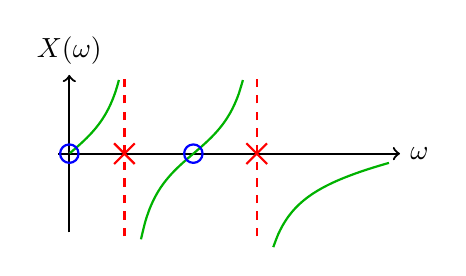
\begin{tikzpicture}[smooth, xscale=0.7, yscale=0.5]
% Achsen
\draw[->, thick] (-0.2,0) -- +(6.2,0) node[right] {$\omega$}; % Horizontal
\draw[->, thick] (0,-2) -- +(0,4) node[above] {$X(\omega)$}; % Vertikal

% Plots
\draw[color=green!70!black, thick] plot[domain=0.01:0.9] (\x, {tan( (\x *1.2) r )        }); % Erster Tan
\draw[color=green!70!black, thick] plot[domain=1.3:3.15] (\x,    {tan( (\x*1.2 -2.7) r)    }); % Erster Tan
\draw[color=green!70!black, thick] plot[domain=6.5:8.6] (\x-2.8,  { ((0.25 * \x) -1/(\x -6)) -2 }); % letzte kurve

% Poolstellen
\draw[dashed, thick, draw=red] (1,-2.1) -- +(0,4.2); % Poolstelle 1
\node[cross out, draw=red, thick] at (1,0) {};

\draw[dashed, thick, draw=red] (3.4,-2.1) -- +(0,4.2); % Poolstelle 2
\node[cross out, draw=red, thick] at (3.4,0) {};



% Nullstellen
\node[rounded rectangle, draw=blue, thick] at(0,0) {};
\node[rounded rectangle, draw=blue, thick] at(2.25,0) {};

\end{tikzpicture}